\documentclass{article}
\usepackage{amsmath}
\usepackage{tikz}
\usepackage{pgfplots}
\pgfplotsset{compat=1.18}
\begin{document}
\section{Shapes}
\begin{center}
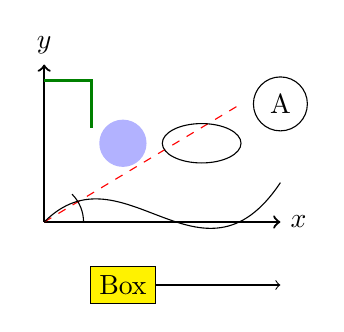
\begin{tikzpicture}
  \draw[thick,->] (0,0) -- (3,0) node[right] {$x$};
  \draw[thick,->] (0,0) -- (0,2) node[above] {$y$};
  \draw[red, dashed] (0,0) -- (2.5,1.5);
  \fill[blue!30] (1,1) circle (0.3);
  \draw (2,1) ellipse (0.5 and 0.25);
  \node[draw, circle] at (3,1.5) {A};
  \node[draw, fill=yellow] (b) at (1,-0.8) {Box};
  \draw[->] (b) -- (3,-0.8);
  \draw (0,0) .. controls (1,1) and (2,-1) .. (3,0.5);
  \draw (0.5,0) arc (0:45:0.5);
  \draw[very thick, green!50!black] (0,1.8) -| (0.6,1.2);
\end{tikzpicture}
\end{center}
\section{Tables}
\begin{center}
\begin{tabular}{|l|c|r|}
\hline
Name & Middle & Value \\
\hline
alpha & $x^2$ & 1.5 \\
longer entry & $\frac{a}{b}$ & 22 \\
\hline
\end{tabular}
\end{center}
\section{Plots}
\begin{figure}[h]
\centering
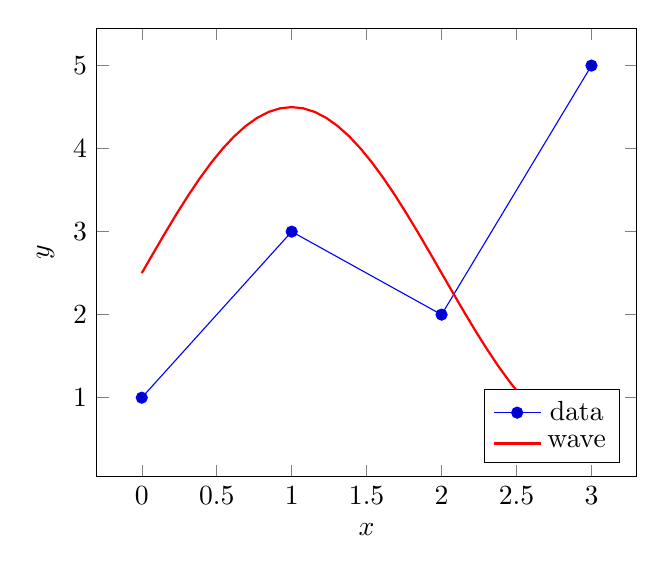
\begin{tikzpicture}
\begin{axis}[xlabel={$x$}, ylabel={$y$}, legend pos=south east]
\addplot coordinates {(0,1) (1,3) (2,2) (3,5)};
\addlegendentry{data}
\addplot[red, thick, domain=0:3, samples=40] {sin(x*90)*2+2.5};
\addlegendentry{wave}
\end{axis}
\end{tikzpicture}
\caption{Automatic limits and ticks.}
\end{figure}
\end{document}
